%
% Routing Strategies
%

\section{Routing strategies} \label{sec:strategies} \index{Routing strategies}

\dropcap{I}{n} Sec.~\ref{sec:costs} we introduced the notion of network costs, strategies for allocating network resources in Sec.~\ref{sec:route_strats}, and a general formalism for optimising strategies so as to minimise costs in Sec.~\ref{sec:strat_opt}. In this section we present some meaningful example strategies and associated pseudo-code fragments, illustrating the implementation of various aspects of strategies of practical real-world interest.

%
% Single User
%

\subsection{Single user} \label{sec:single_user_shortest} \index{Single user strategies}

Let us begin our discussion of strategies by considering the simplest case of just a single user on the network. Consider the graph shown in Fig.~\ref{fig:simp_route_opt}. This is the same example used earlier, but now the edges have been weighted by some arbitrary cost metric. There are four routes from $A$ to $B$. All have cost \mbox{$c=3$} except the route indicated by the red arrow, which has cost \mbox{$c=2$}. Clearly the latter is optimal in terms of cost minimisation, and any shortest-path algorithm applied between $A$ and $B$ will accurately come to that conclusion. Thus, single-user networks are very trivial to optimise, and there is no distinction between \textsc{Local} and \textsc{Global} strategies.

The very trivial algorithm for this route finding is shown in Alg.~\ref{alg:single_user}, where the \texttt{ShortestPath()} function could be any of the existing, well-known shortest path algorithms (Sec.~\ref{sec:shortest_path}).
\begin{table}[!htbp]
\begin{mdframed}[innertopmargin=3pt, innerbottommargin=3pt, nobreak]
\texttt{ 
function Strategy.SingleUser(Packets):
\begin{enumerate}
    \item for(packet$\in$Packets) \{
        \setlength{\itemindent}{.2in}
                \item currentNode = packet.RoutingQueue.Pop()
        \item shortestRoute = \\
        ShortestPath(currentNode,packet.Recipient)
        \item packet.RoutingQueue.Flush()
        \item packet.RoutingQueue.Push(shortestRoute)
    \setlength{\itemindent}{0in}
    \item \}
    \item $\Box$
\end{enumerate}}
\end{mdframed}
\captionspace \caption{For a single user, a simple shortest-path algorithm necessarily finds the optimal route, as there is no potential for packet collisions or competition for network resources.} \label{alg:single_user}
\end{table}

%
% Multiple Users
%

\subsection{Multiple users} \label{sec:two_user} \index{Multiple user strategies}

Next consider the more complex network shown in Fig.~\ref{fig:conflict}. We consider two sender/receiver pairs, \mbox{$A_1\to B_1$} and \mbox{$A_2\to B_2$}. The available routes connecting both pairs overlap, creating competition for network resources.

Let us assume there are just two properties of interest when deciding strategies -- cost in dollars (which may differ for different links), and availability (i.e how many states can the channel handle at once). Let $c_1$ be the dollar cost, and \mbox{$a_1$} be the amount of available channel capacity. Our network is very primitive and each channel can only accommodate one state at a time. Thus, we let \mbox{$a_1=1$} for all links, except for the one common to both $R_1$ and $R_3$, \mbox{($R_1\cap R_3$)}, which we invest more heavily into, since both routes are going to be wanting to use this link.

To define our net cost measure, we combine $c_1$ and $a_1$ according to,
\begin{align}
\mathcal{S} : f_\mathrm{net}(\vec{c}) = \left\{
\begin{array}{l l}
c_1 & \quad \mathrm{if}~ a_1>0 \\
\infty & \quad \mathrm{if}~~ a_1=0 \\
\end{array} \right..
\end{align}
That is, provided bandwidth is available, the link will have the dollar cost $c_1$. If no bandwidth is available, the cost is infinite, thereby removing the respective link from the graph.

Next the cost metrics are updated by the strategy $\mathcal{S}$ following each communication. In this instance this simply decrements the bandwidth attribute for the links that were utilised,
\begin{align}
\mathcal{S} : a_1 \to a_1-1.
\end{align}

Suppose the strategy optimises the \mbox{$A_1\to B_1$} route first, yielding $R_3$, before moving onto the \mbox{$A_2\to D_2$} route. In this case, the reduction of the bandwidth attribute signals that the cheapest route $R_2$ is no longer available to be utilised simultaneously to $R_3$, and must therefore wait its turn on the following clock-cycle. Alternately, the strategy could employ $R_1$ for \mbox{$A_2\to B_2$}, in which case their common link with capacity for two states would eliminate the competition between the two communications, allowing both to take place simultaneously. Thus, there is a tradeoff: for \mbox{$A_2\to B_2$}, we could achieve a net cost of \mbox{$c(A_2\to B_2)=5$}, requiring 2 clock-cycles; or we could achieve simultaneous communication at the expense of increasing cost to \mbox{$c(A_2\to B_2)=6$}. This indicates that when choosing strategies, we must carefully define its goals.

Suppose net cost, rather than clock-cycles, was the key measure of interest. Then choosing the routes $R_1$ and $R_3$ would be the optimal choice. An optimal \textsc{Global} optimisation would recognise this. However, a \textsc{Local} optimisation, based on choosing shortest-paths one-by-by for each sender/receiver pair, may or may not choose the optimal routes, depending on the order in which the decisions were made.

Suppose the \mbox{$A_2\to B_2$} route were optimised first. We would choose $R_2$. Then there would be a traffic jam on the \mbox{$A_1\to B_1$} route, and it would necessarily have to wait its turn. In a time-critical application, where waiting is intolerable, this effectively renders the network useless to the first sender/receiver pair.

If, however, the \mbox{$A_1\to B_1$} were optimised first, choosing $R_3$, then $R_2$ would be prohibited once the bandwidth attributes were updated, and the second best option, $R_1$, would be chosen. Now both communications could take place simultaneously. So we see that the outcomes of \textsc{Local} optimisations needn't always be consistent or unique. Rather, they can be highly dependent upon circumstantial issues, such as the arbitrary order in which routes are chosen for optimisation.

\begin{figure}[!htbp]
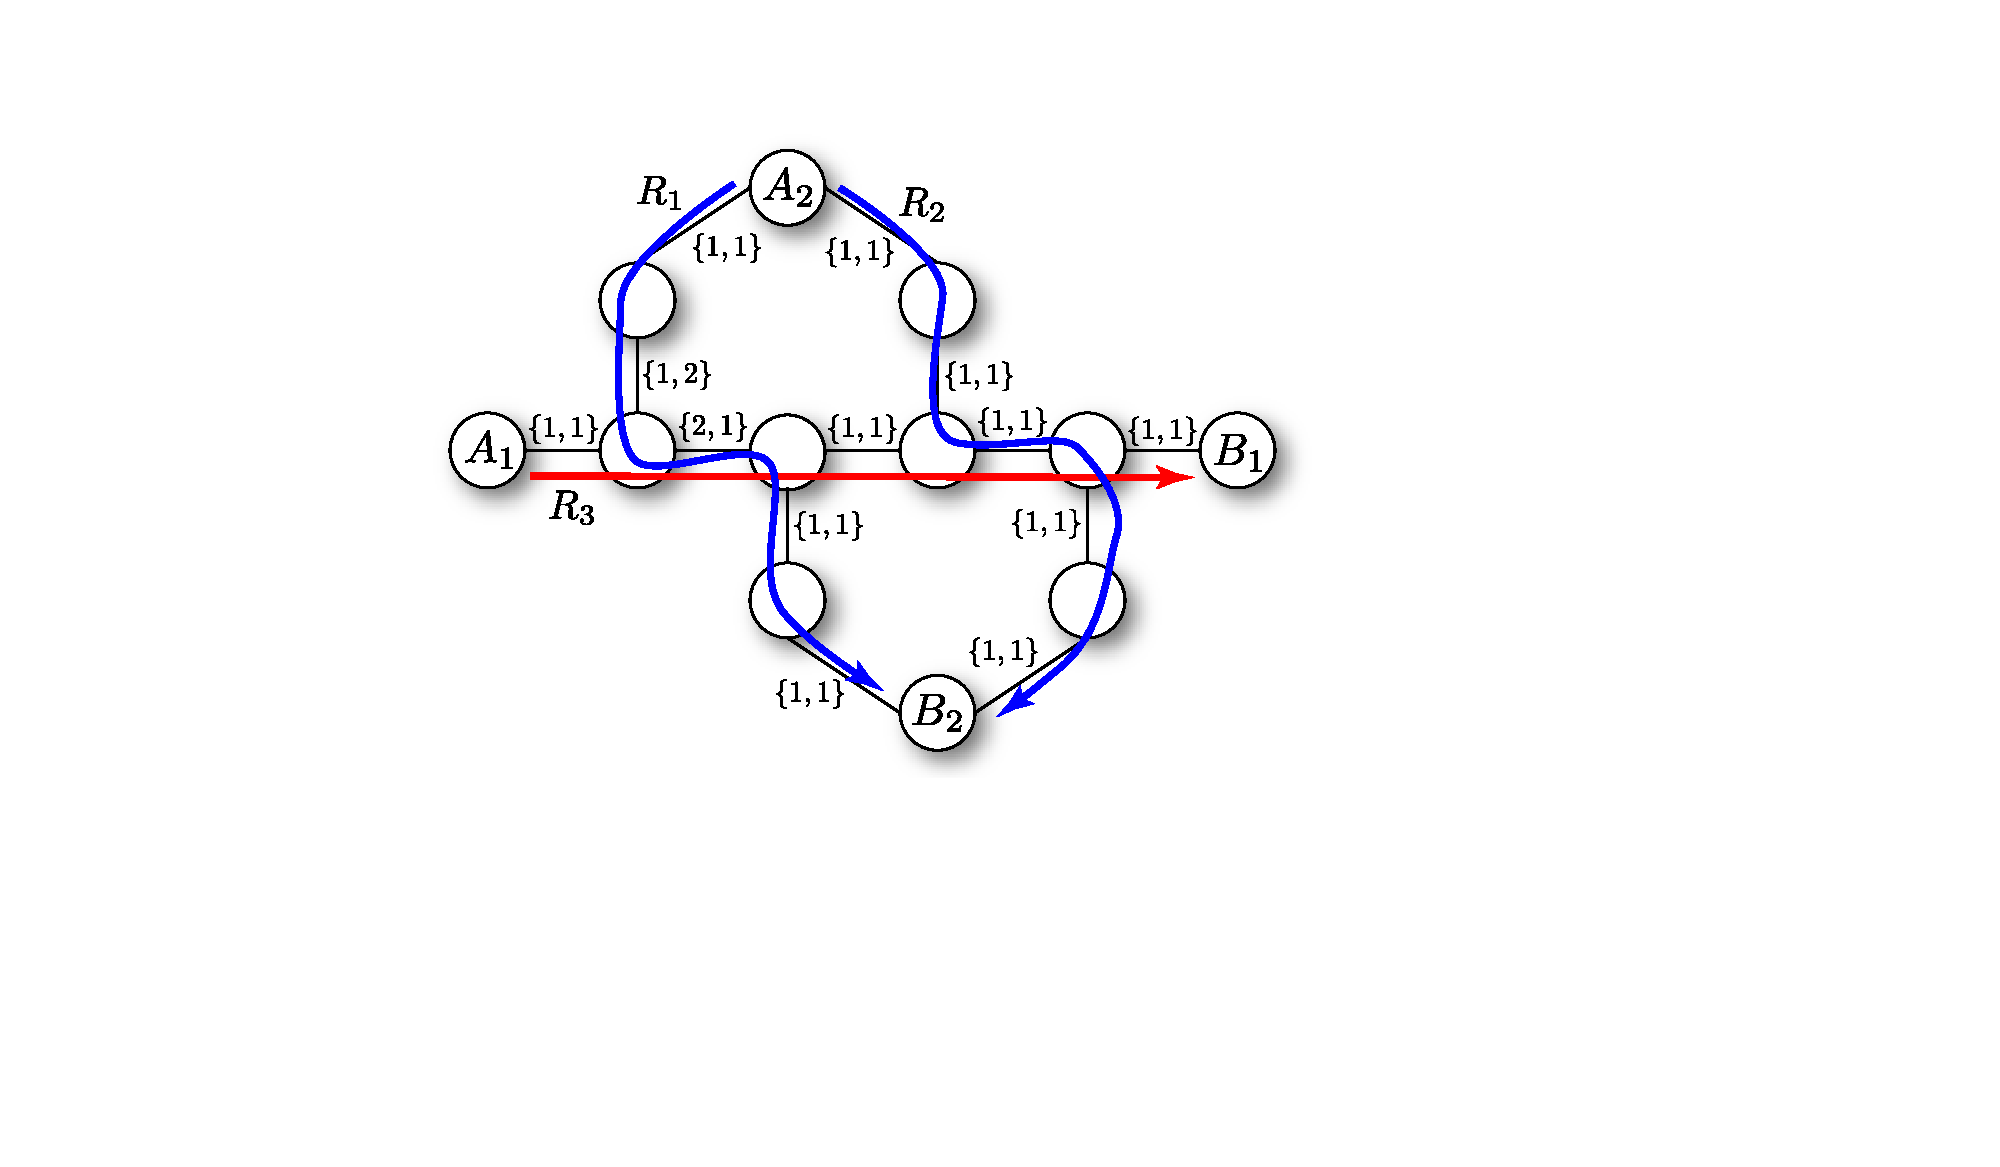
\includegraphics[width=0.475\textwidth]{conflict}
\captionspace \caption{A simple network with two competing pairs of senders and receivers, \mbox{$A_1\to B_1$} and \mbox{$A_2\to B_2$}. Edges are labelled by \mbox{$\{b,d\}$}, where $b$ is the bandwidth attribute of the link (i.e number of states that can be communicated simultaneously), and $d$ is the cost metric associated with the link, e.g loss in dB. (blue line) $R_1$ and $R_2$ are two routes from $A_2\to B_2$. Either of these routes could be declared optimal, depending on the choice of cost function. For a trivial additive cost function, $R_2$ would be declared optimal. (red lines) $R_3$ is the optimal route from \mbox{$A_1\to B_1$}.} \label{fig:conflict}
\end{figure}

Generalising this to any number of users is a straightforward extension to the route optimisation problem, incurring a higher computational overhead due to the increased optimisation complexity.

In the upcoming sections we discuss multi-user strategies in more detail. None of these are true \textsc{Global} strategies, but nonetheless address some of the problems facing \textsc{Local} strategies mentioned above.

Truly \textsc{Global} strategies could employ, for example, the vehicle routing problem (Sec.~\ref{sec:VRP}) or vehicle rescheduling problem (Sec.~\ref{sec:VRSP}) algorithms. However, both of these are \textbf{NP}-hard\index{NP \& NP-complete} in general. Thus, the approximation heuristics to be discussed in the following sections are highly applicable.

%
% Round Robin
%

\subsection{Round robin} \label{sec:round_robin} \index{Round robin strategies}

Perhaps the simplest and most elegant multi-user scheduling strategy is to borrow from the idea of time-division multiplexing for preemptive multitasking employed by UNIX operating systems. Here we simply put all live packets in a list, and go through the list, one-by-one, giving each packet an equal time-share of network resources, independent of costs. The algorithm for this is shown in Alg.~\ref{alg:round_robin}.

\begin{table}[!htbp]
\begin{mdframed}[innertopmargin=3pt, innerbottommargin=3pt, nobreak]
\texttt{
function Strategy.RoundRobin(Packets):
\begin{enumerate}
    \item for(packet$\in$Packets) \{
        \setlength{\itemindent}{.2in}
                \item currentNode = packet.RoutingQueue.Pop()
        \item shortestRoute = \\
        ShortestPath(currentNode,packet.Recipient)
        \item packet.RoutingQueue.Flush()
        \item packet.RoutingQueue.Push(shortestRoute)
    \setlength{\itemindent}{0in} \}
    \item $\Box$
\end{enumerate}}
\end{mdframed}
\captionspace \caption{In the \textsc{Round Robin} strategy we simply iterate through the list of active packets, with no regard for any metrics, or conflicts between them. Rather, we strive for perfect time-sharing equality, and every packet entirely ignores the actions of all other packets, performing a completely selfish optimisation strategy.} \label{alg:round_robin}
\end{table}
The \textsc{Round Robin} strategy can be considered base skeleton code for more sophistic algorithms to build upon, simply by reordering the packet queue.

While such a protocol clearly ensures scheduling that gives all packets attention, it is the perfect example of an algorithm subject to the resource allocation imbalance discussed in Sec.~\ref{sec:two_user}. Specifically, the routes being followed by some packets may systemically receive more favourable treatment than others, based on the arbitrary ordering of the list of packets. Also, equal timesharing fails to accommodate for the fact that some routes are inherently more costly than others and deserve a greater share of network resources.

%
% Data Priority
%

\subsection{Data priority} \label{sec:data_priority} \index{Data priority strategies}

Are all men created equal? No. Some packets may inherently be more important than others, and ought to receive priority when allocating network resources. A simple variation on the \textsc{Round Robin} strategy is to, before iterating through the list of packets, order them according to a \textsc{Priority} attribute. Thus, when applying a shortest-path algorithm, it is deemed most important to minimise the costs of the more important packets first.

This is trivially achieved by taking the existing \textsc{Round Robin} strategy, and first ordering the packet list by their priority attributes, i.e by inserting a new line 1, \mbox{\texttt{Packets.SortByPriority()}}.

%
% Randomisation
%

\subsection{Randomisation} \label{sec:random} \index{Randomised strategies}

The imbalance issue facing the \textsc{Round Robin} strategy (Sec.~\ref{sec:round_robin}) may be most trivially addressed using randomisation of the strategy, such that routes are optimised in an order chosen randomly each time. This would allow the different sender/receiver pairs to have equal access to network resources, when averaged over many network uses.

This is also a straightforward variation of the \textsc{Round Robin} strategy, achieved by first randomising the list of packets before the other stages, i.e insert a new line 1, \mbox{\texttt{Packets.RandomizeOrder()}}.

%
% Cost Priority
%

\subsection{Cost priority} \label{sec:cost_priority} \index{Cost priority strategies}

The \textsc{Random} strategy overcomes one key problem facing any \textsc{Local} optimisation strategy. But it is nonetheless merely a mild variation on the \textsc{Round Robin} strategy, guaranteeing equal time-share to each sender/receiver pair. But does equal time-sharing actually represent the best allocation of resources?

It isn't just the order in which routes are chosen, which creates imbalance between users. The costs and attributes of the routes themselves is inevitably biased more in favour of some users than others. To accommodate this we now introduce the \textsc{Cost Priority} strategy. Here, rather than prioritising packets on a random basis, or according to a fixed, predetermined priority attribute, we do so according to their net accumulated cost. Those who have accumulated the highest cost will subsequently be treated with highest priority. This strategy effectively introduces a negative feedback loop into resource allocation, creating a self-regulating (and hopefully stable!) time-multiplexed packet-switched network. The pseudo-code for the \textsc{Cost Priority} strategy is shown in Alg.~\ref{alg:cost_prior_alg}.

\begin{table}[!htbp]
\begin{mdframed}[innertopmargin=3pt, innerbottommargin=3pt, nobreak]
\texttt{
function Strategy.CostPriority(Packets):
\begin{enumerate}
    \item packetsAndCosts = []
    \item for(packet$\in$Packets) \{
        \setlength{\itemindent}{.2in}
        \item cost = costFunction(packet)
        \item packetsAndCosts.Append([packet,cost])
    \setlength{\itemindent}{0in}
    \item     \}
    \item sorted = \\
        SortByCostDescending(packetsAndCosts)
    \item for(packet$\in$sorted) \{
        \setlength{\itemindent}{.2in}
        \item currentNode = packet.RoutingQueue.Pop()
        \item shortestRoute = \\
        ShortestPath(currentNode,packet.Recipient)
        \item packet.RoutingQueue.Flush()
        \item packet.RoutingQueue.Push(shortestRoute)
    \setlength{\itemindent}{0in}
    \item \}
    \item $\Box$
\end{enumerate}}
\end{mdframed}
\captionspace \caption{The \textsc{Cost Priority} strategy scheduling algorithm that gives highest routing priority to \textsc{Packets} with the highest accumulated cost (i.e which have suffered the most). The as-yet undefined \texttt{costFunction()}, which refers to $f_\mathrm{cost}$ from Eq.~(\ref{eq:net_cost_R}), is where the details of the priority decisions are made, which could be entirely arbitrary. In this example, the shortest route is recalculated at each step, based on the expectation that network metrics are dynamic.} \label{alg:cost_prior_alg}
\end{table}

This is an example of a \textsc{Greedy} optimisation algorithm, which attempts to optimise routing by always optimising the most desperate packets first, in descending order down to the least. It is well-known that \textsc{Greedy} algorithms often do not find global optima. Nonetheless, this approach improves on the previous multi-user protocols.

Let us consider a simple example scenario. Imagine we begin with an ordinary network graph, with edges weighted by costs and attributes. For generality, we will additionally assume the available network resources are very dynamic and unpredictable. The costs associated with links are at the whim of market forces we do not understand (do we ever?). And, for the sake of example, and to make matters worse, the links have been very unreliable lately, and are routinely dropping in and out -- `blackouts'. This effectively rules out \textit{a priori} route optimisation, requiring something dynamic.

There are many users on the network, with many active packets at any give time, but because of the constant oscillations in network resources, some packets have received second-class treatment, and through neglect accumulated an unfair share of state degradation. This simple toy model is, at least qualitatively, something that could arise quite naturally in networks with constrained or unreliable resources.

Let us define an example \textsc{Cost Priority} strategy using the following:
\begin{itemize}
\item \textsc{Latency} cost: How long has the packet has been in transit for? This is actually a very general cost metric, since any other cost metric measured in units per time will be directly proportional to this metric. That is, loss, fidelity, purity, efficiency, and so on, all mirror this metric when expressed on a decibel scale. Of course, the same strategy could have easily been applied to any other cost metric.
\item \textsc{Blackout} attribute: Is our unreliable link actually working right now? A given link will have probability $p_\mathrm{op}$ of being operational at any given time, chosen independently for each link at each clock-cycle. The \texttt{Attributes.Update()} function from Alg.~\ref{alg:transport_alg} is responsible for implementing this.
\item \mbox{\textsc{Cost Function}} ($f_\mathrm{cost}$, \texttt{costFunction()} in Alg.~\ref{alg:cost_prior_alg}): The strategy must make sensible decisions based upon only the above two parameters. Because of the previously mentioned generality of the \textsc{Latency} metric, we would like the net cost to directly reflect this metric, but only of course, if the link is operational. If it is not, then that link must be ruled out entirely by assigning it an infinite cost. Thus, we simply choose,
\begin{align}
\mathcal{S} : f_\mathrm{cost}(c,a) = \left\{
\begin{array}{l l}
c & \quad \mathrm{if}~ a=\mathrm{\texttt{True}} \\
\infty & \quad \mathrm{if}~ a=\mathrm{\texttt{False}} \\
\end{array} \right..
\end{align}
Note that different packets could be associated with different net cost functions, $f_\mathrm{net}$, to accommodate for the different QoS requirements of different users and messages.
\end{itemize}

In other words, the net cost is taken directly from the underlying cost metric, and modulated by an attribute, yielding a net cost for each packet, which is used to determine which packets receive priority.

This provides us with a simple illustration of how costs and attributes can compliment one another to yield meaningful strategies, that improve network performance over na\"ive, but well-intentioned, time-sharing approaches.

%
% All or Nothing
%

\subsection{All or nothing} \label{sec:all_or_nothing} \index{All or nothing strategies}

In some cases, end-user applications may have strict QoS constraints associated with any data they receive. For example, in a time-critical enterprise, say high-frequency trading, receiving information a millisecond too late is worthless, and it would be best to discard the out of date information to free up bandwidth for the next round of information. Alternately, if the fidelity of a state is required to strictly fall within a fault-tolerance threshold, it will be useless if the threshold is violated. In such a context, the \textsc{Strategy} will apply hard boundaries on QoS metrics, discarding anything violating it, after which some other \textsc{Strategy} is applied. The algorithm is summarised in Alg.~\ref{alg:all_or_nothing}.

\begin{table}[!htbp]
\begin{mdframed}[innertopmargin=3pt, innerbottommargin=3pt, nobreak]
\texttt{
function Strategy.AllOrNothing(Packets, threshold):
\begin{enumerate}
    \item for(packet$\in$Packets) \{
        \setlength{\itemindent}{.2in}
        \item cost = packet.costFunction()
        \item if(cost $\geq$ threshold) \{
        \setlength{\itemindent}{.4in}
            \item packet.Sender.Notify(\textsc{Failure})
            \item packet.Recipient.Notify(\textsc{Failure})
            \item packet.Discard()
                    \setlength{\itemindent}{.2in}
            \item \}
        \setlength{\itemindent}{0in}
    \item \}
    \item Strategy.SomeOtherStrategy(Packets)
    \item $\Box$
\end{enumerate}}
\end{mdframed}
\captionspace \caption{The \textsc{All or Nothing} strategy. If the net cost of a packet exceeds a certain \texttt{threshold}, it is discarded outright, and the sender and recipient notified.} \label{alg:all_or_nothing}
\end{table}

%
% Optimal Flow
%

\subsection{Optimal flow} \index{Optimal flow strategies}

In Sec.~\ref{sec:flow_networks} we introduced flow networks as a means for analysing networks where maximising network flow (throughput) is the primary objective. Formulating our quantum networks in this manner is extremely convenient since, combined with our existing definitions for cost metrics and attributes, we can easily exploit a plethora of known results from flow network theory.

As an example of how load allocation might be applied in a simple network, consider again the network shown in Fig.~\ref{fig:simp_route_opt}, where the edge weights are regular cost metrics (not capacities). Alice wishes to send two packets to Bob, simultaneously if possible. Clearly she would transmit her first packet over the \mbox{$A\to F\to B$} route, since this has lowest cost. But let us assume that every link has a maximum capacity of one packet per unit time. In this case Alice will be unable to send her second packet via the same route and must instead resort to using \mbox{$A\to C \to B$} or \mbox{$A\to D\to B$}. The optimisation is straightforward in this instance. However, in general these types of optimisations are somewhat more involved.

These scenarios are handled by flow network optimisation algorithms, of which there are many. We discuss a few of the most relevant ones for our purposes in Sec.~\ref{sec:graph_theory}. Note that these algorithms are \textsc{Global} optimisation algorithms, requiring complete knowledge of the status of the entire network to perform the optimisation.

The routing strategy is very straightforward, shown in Alg.~\ref{alg:opt_flow}, since the \textsc{Global} flow-optimisation algorithm completely specifies the entire configuration of routes through the network.

\begin{table}[!htbp]
\begin{mdframed}[innertopmargin=3pt, innerbottommargin=3pt, nobreak]
\texttt{
function Strategy.OptimalFlow(Packets):
\begin{enumerate}
    \item routes = Packets.OptimalFlowRoutes()
    \item for(packet$\in$Packets) \{
        \setlength{\itemindent}{.2in}
                \item packet.RoutingQueue.Flush()
                \item packet.RoutingQueue.Push(routes[packet])
                \setlength{\itemindent}{0in} 
    \item \}
    \item $\Box$
\end{enumerate}}
\end{mdframed}
\captionspace \caption{A generic optimal flow routing strategy. \textsc{Packets} is the array of all packets that ought to be transmitted simultaneously, which are collectively optimised using some flow optimisation algorithm before undergoing transport.} \label{alg:opt_flow}
\end{table}